  \pagebreak
  \subsection{Análisis de una señal modulada en amplitud} \label{sec:Exp4_AM}
    Las señales que son moduladas en amplitud (AM) poseen un espectro característico, como el que se puede ver
    en la Figura~\ref{fig:EjemploEspectroModAM}. Mediante el espectro se puede medir frecuencia, pero también
    las amplitudes, de portadora y bandas laterales, lo que permite calcular el índice de modulación, el cual es
    un parámetro importante a tener en cuenta. 

    \begin{figure}[H]
      \centering
      \frame{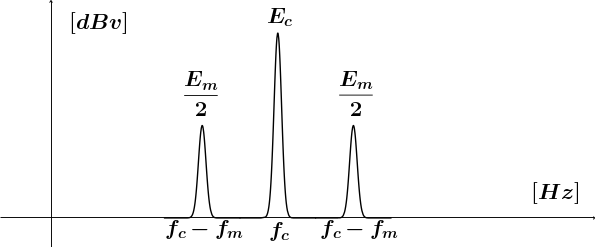
\includegraphics[width=0.48\textwidth]{Imagenes/ActividadPractica/4AnalisisDeUnaSeñalDeAM/EjemploEspectroAM.png}}
      \caption{Ejemplo de espectro de una señal AM.}
      \label{fig:EjemploEspectroModAM}
    \end{figure}

    Recordando que el índice de modulación es $m= E_m / Ec$, y además, que el módulo matemático del osciloscopio 
    en cuestión mide las amplitudes en dBv, entonces

    \begin{equation}
      m = \dfrac{E_{BLalteral} \cdot 2}{E_{Portadora}} \hspace{20pt}
      \Longrightarrow \hspace{20pt} m_{dB} = dBv_{BLateral} - dBv_{Portadora} + 6dB
      \label{eqn:IndiceModEndB}
    \end{equation}

    \begin{equation}
      \therefore \hspace{20pt} m=10^{\dfrac{m_{dB}}{20}}
      \label{eqn:IndiceMod}
    \end{equation}

    Para poder visualizar el espectro de una señal AM se utiliza el circuito de la Figura~\ref{fig:ModuladorAM}. 
    El mismo posee una circuito sintonizado o resonante, el cual está diseñado para que su
    frecuencia sea de $\mathbf{f_o = 50~kHz}$.

    \begin{figure}[H]
      \centering
      \frame{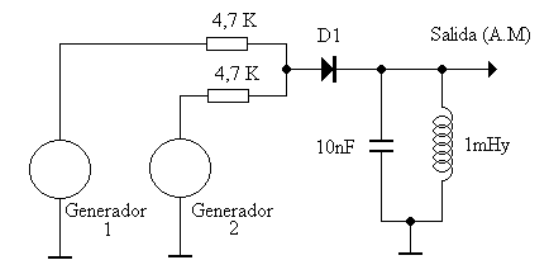
\includegraphics[width=0.48\textwidth]{Imagenes/ActividadPractica/4AnalisisDeUnaSeñalDeAM/CircuitoModAM.png}}
      \caption{Circuito de modulación en amplitud.}
      \label{fig:ModuladorAM}
    \end{figure}

    Con el generador \textbf{G1} se inyecta una señal senoidal que actúa como \textbf{portadora} de frecuencia 
    $\mathbf{f_c=50~kHz}$, y con el generador \textbf{G2} se inyecta la señal \textbf{modulante} de frecuencia
    $\mathbf{f_m=1~kHz}$, que puede ser senoidal, triangular o cuadrada. Las amplitudes utilizadas mantienen 
    una relación tal que la de la portadora sea el doble que la de modulante.

    \subsubsection{Señal senoidal como modulante}
      Se setea el generador G2 para que entregue una señal senoidal, que actúa como banda base. Dicha señal
      y la portadora se pueden ver en la Figura~\ref{fig:SeñalesParaAM1}.
      
      \begin{figure}[H]
        \centering
        \begin{subfigure}[H]{0.48\textwidth}
          \frame{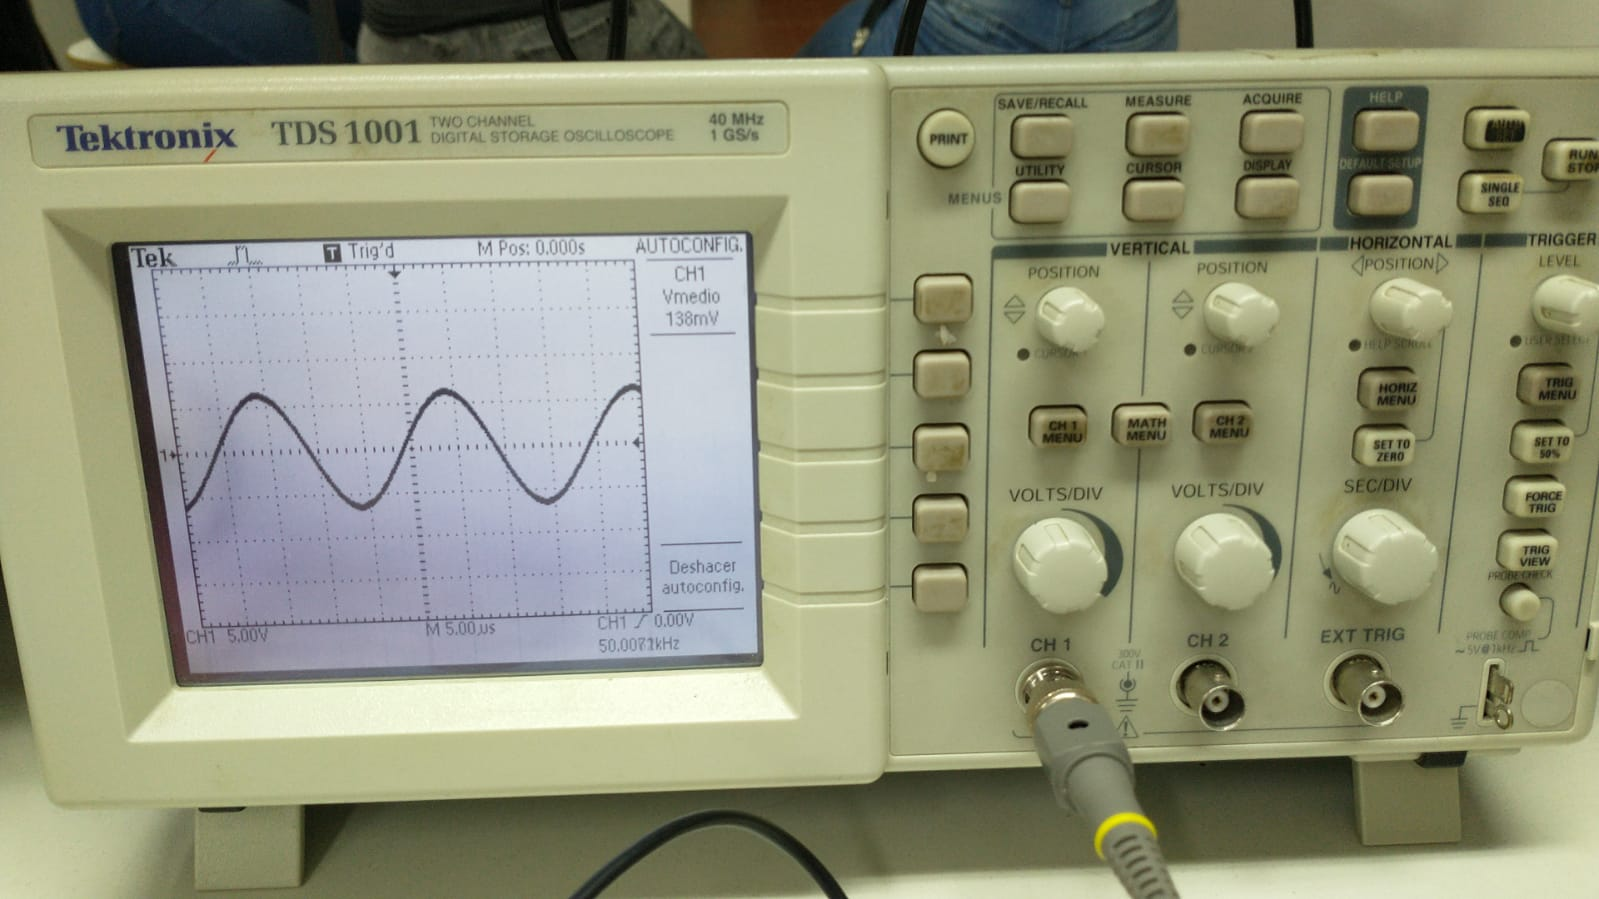
\includegraphics[width=\textwidth]{Imagenes/ActividadPractica/4AnalisisDeUnaSeñalDeAM/Exp4_G1Portadora_enTiempo.jpeg}}
          \caption{Portadora.}
          \label{fig:PortadoraEnTiempo}
        \end{subfigure}
        \hfill 
        \begin{subfigure}[H]{0.45\textwidth}
          \frame{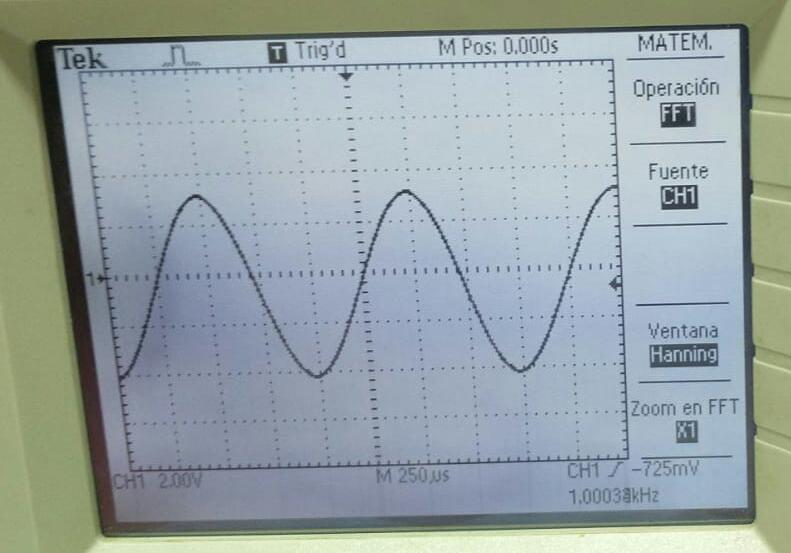
\includegraphics[width=\textwidth]{Imagenes/ActividadPractica/4AnalisisDeUnaSeñalDeAM/Exp4_G2SenoModulante_enTiempo.jpeg}}
          \caption{Banda base senoidal.}
          \label{fig:SenoModulanteEnTiempo}
        \end{subfigure}
      
        \caption{Señales utilizadas para modular en amplitud,}
        \label{fig:SeñalesParaAM1}
      \end{figure}
        
      
      Se elige una base de tiempos de $\mathbf{1~ms/div}$ y luego, el menú del trigger se setea de la siguiente manera:
      \textbf{Flanco positivo}, \textbf{CH1}, \textbf{Auto}, \textbf{Rechazo AF}. Con
      todo esto, la imagen obtenida se encuentra en la Figura~\ref{fig:SeñalAM1EnTiempo}.
      
      \begin{figure}[H]
        \centering
        \frame{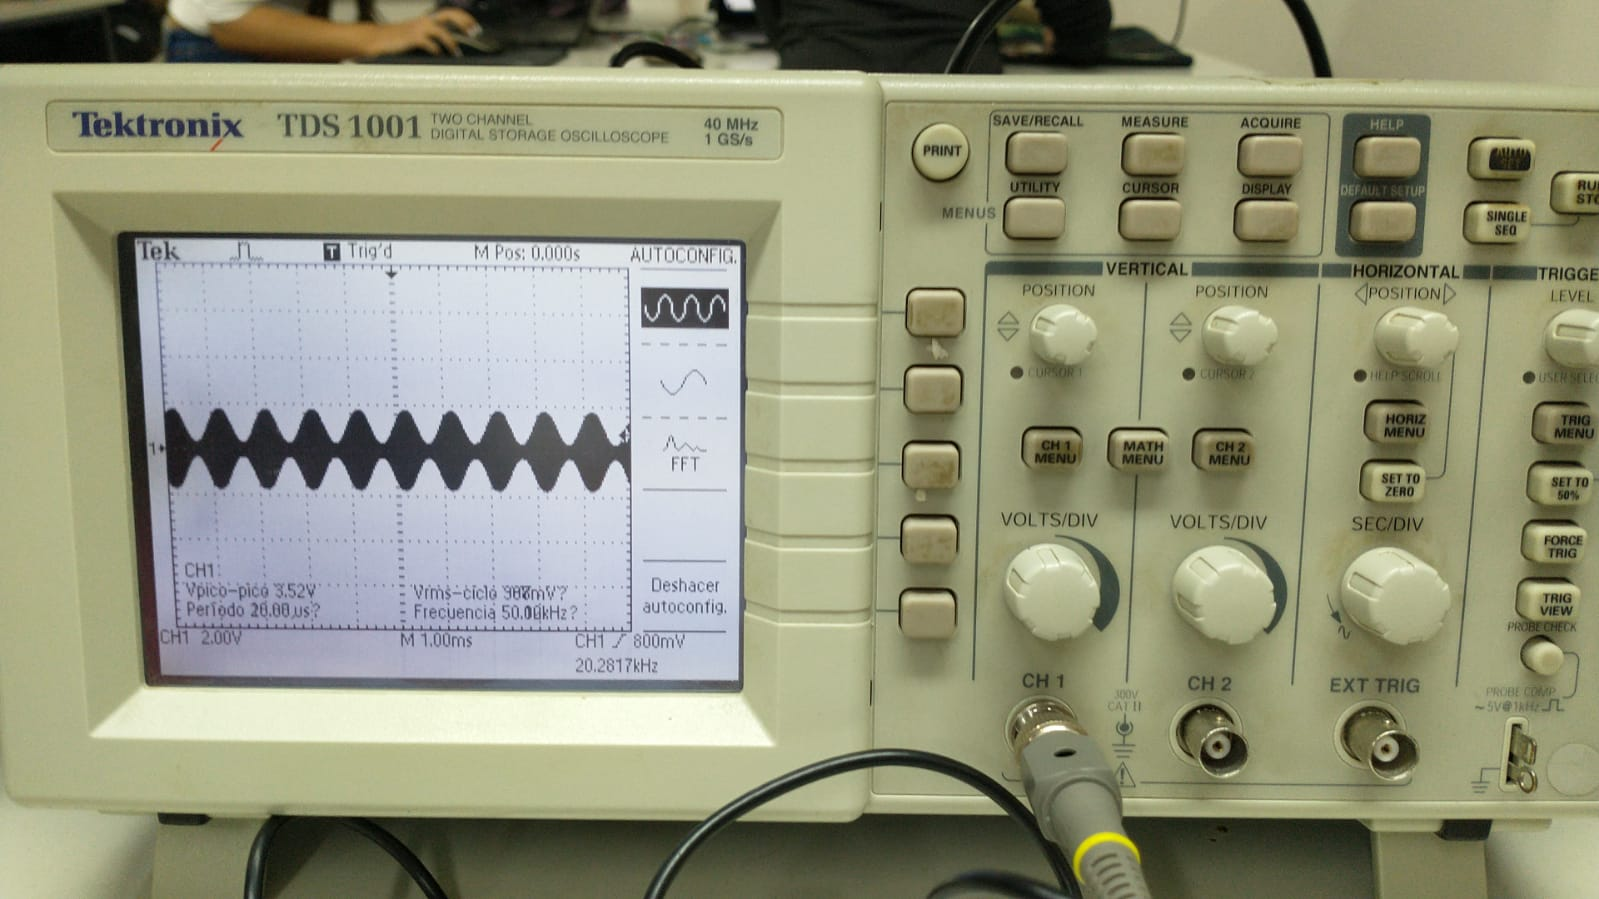
\includegraphics[width=0.48\textwidth]{Imagenes/ActividadPractica/4AnalisisDeUnaSeñalDeAM/Exp4_SeñalAM.jpeg}}
        \caption{Señal AM con seno como modulante.}
        \label{fig:SeñalAM1EnTiempo}
      \end{figure}

      Luego, en el menú matemático se eligen las siguientes opciones: \textbf{FFT}, \textbf{CH1},
      \textbf{Hanning} y \textbf{Zoom x10}. Además, el modo de adquisición se pone en \textbf{Promedio} con 
      64 cuentas. A continuación, mediante el uso de cursores, se procede a medir la frecuencias. Dichas mediciones se 
      pueden apreciar en la Figura~\ref{fig:FreqAMSeno}, y los valores se encuentran tabulados en la 
      Tabla~\ref{tab:MedicionesFreqAMSeno}.

      \begin{figure}[H]
        \centering
        \begin{subfigure}[H]{0.48\textwidth}
          \frame{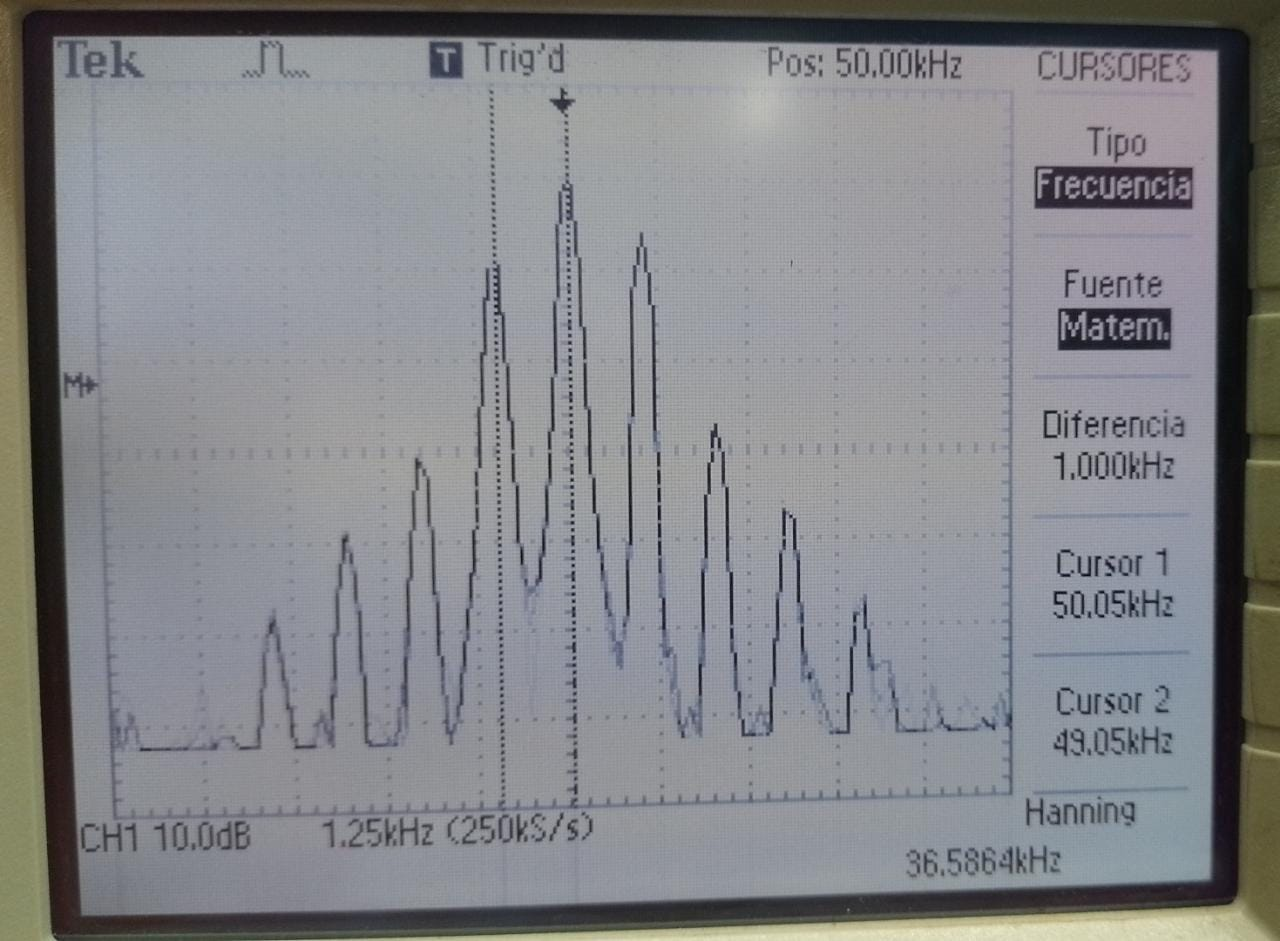
\includegraphics[width=\textwidth]{Imagenes/ActividadPractica/4AnalisisDeUnaSeñalDeAM/Exp4_SeñalAM_MedicionFreqBLInf.jpeg}}
          \caption{Frecuencia BLInf.}
          \label{fig:FreqBLInfAMSeno}
        \end{subfigure}
        \hfill 
        \begin{subfigure}[H]{0.48\textwidth}
          \frame{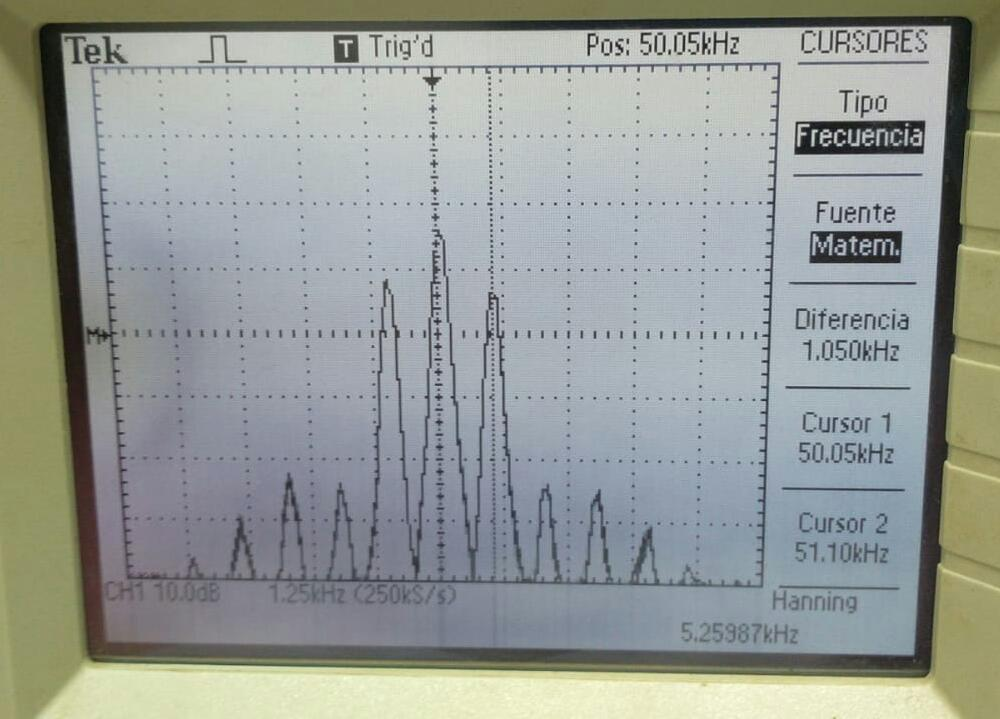
\includegraphics[width=\textwidth]{Imagenes/ActividadPractica/4AnalisisDeUnaSeñalDeAM/Exp4_SeñalAM_MedicionFreqBLSup.jpeg}}
          \caption{Frecuencia BLSup.}
          \label{fig:FreqBLSupAMSeno}
        \end{subfigure}
      
        \caption{Frecuencias de la señal AM con el seno como modulante.}
        \label{fig:FreqAMSeno}
      \end{figure}

      \begin{table}[H]
        \centering
      \begin{tabular}{cccc} \hline \hline
          $\mathbf{f_c} $        &   $\mathbf{f_{BLSup}}$   &   $\mathbf{f_{BLInf}}$    &   $\mathbf{f_m}$  \\ \hline
          $50,05~kHz$   &   $51,05~kHz$   &    $49,05~kHz$   &   $1,00~kHz$   \\ \hline \hline
        \end{tabular}
        \caption{Frecuencias medidas del espectro de la señal AM.}
        \label{tab:MedicionesFreqAMSeno}
      \end{table}

      De la misma forma, se procede a realizar mediciones de amplitud de la señal AM en cuestión. En la
      Figura~\ref{fig:AmplitudesAMSeno} se pueden observar dichas mediciones. Luego, con estas y 
      el uso de las ecuaciones~(\ref{eqn:IndiceModEndB}) y (\ref{eqn:IndiceMod}), se completa la 
      Tabla~\ref{tab:MedicionesAmplitAMSeno}.

      \begin{figure}[H]
        \centering
        \begin{subfigure}[H]{0.48\textwidth}
          \frame{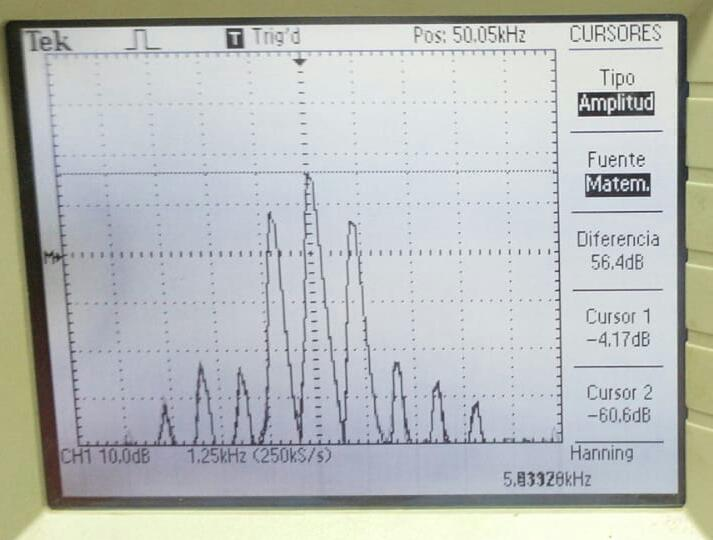
\includegraphics[width=\textwidth]{Imagenes/ActividadPractica/4AnalisisDeUnaSeñalDeAM/Exp4_SeñalAM_MedicionAmplPortadora.jpeg}}
          \caption{Amplitud Portadora.}
          \label{fig:AmplitudBLInfAMSeno}
        \end{subfigure}
        \hfill 
        \begin{subfigure}[H]{0.48\textwidth}
          \frame{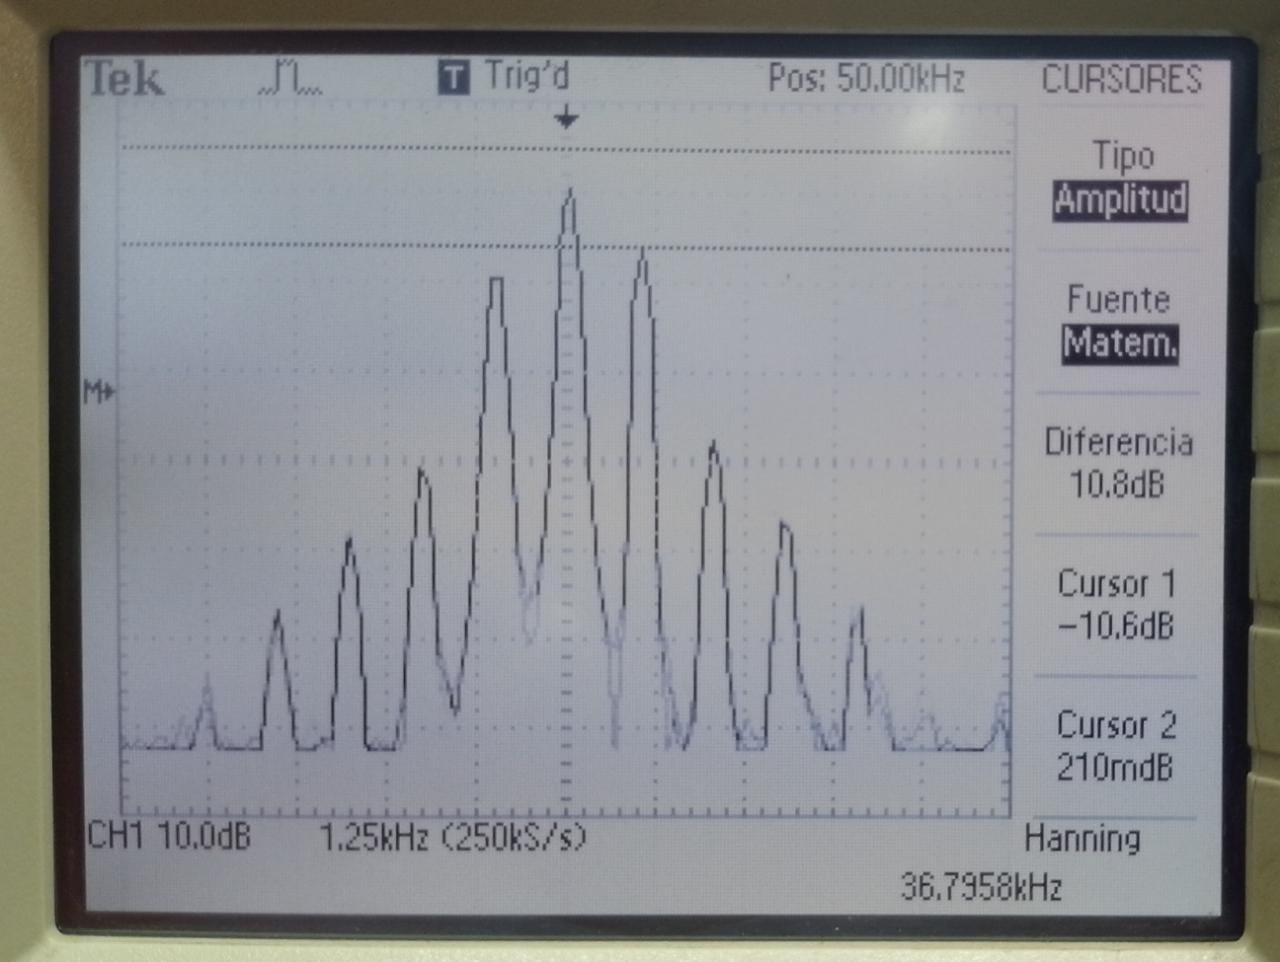
\includegraphics[width=\textwidth]{Imagenes/ActividadPractica/4AnalisisDeUnaSeñalDeAM/Exp4_SeñalAM_MedicionAmplBLSup.jpeg}}
          \caption{Amplitud BLSup.}
          \label{fig:AmpltiudBLSupAMSeno}
        \end{subfigure}
      
        \caption{Amplitudes de la señal AM con el seno como modulante.}
        \label{fig:AmplitudesAMSeno}
      \end{figure}


      \begin{table}[H]
        \centering
      \begin{tabular}{cccc} \hline \hline
          \textbf{Ampl. BLSuperior}    &   \textbf{Ampl. Portadora}  &  \textbf{Índice m}  & \textbf{Índice m}  \\ \hline
          $-4,59~dBv$   &   $-10,60~dBv$   &    $-9,19~dB$   &   $0,35$   \\ \hline \hline
        \end{tabular}
        \caption{Amplitudes medidas e índice de modulación.}
        \label{tab:MedicionesAmplitAMSeno}
      \end{table}


    \subsubsection{Señal cuadrada como modulante}
      A continuación, se procede a cambiar el generador \textbf{G2} para que inyecte una la señal cuadrada
      como \textbf{modulante} con la misma frecuencia antes utilizada, respetando la relación de amplitudes
      previamente configurada. La señal AM obtenida se puede ver en la Figura~\ref{fig:SeñalAMConCuadrada}.

      \begin{figure}[H]
        \centering
        \frame{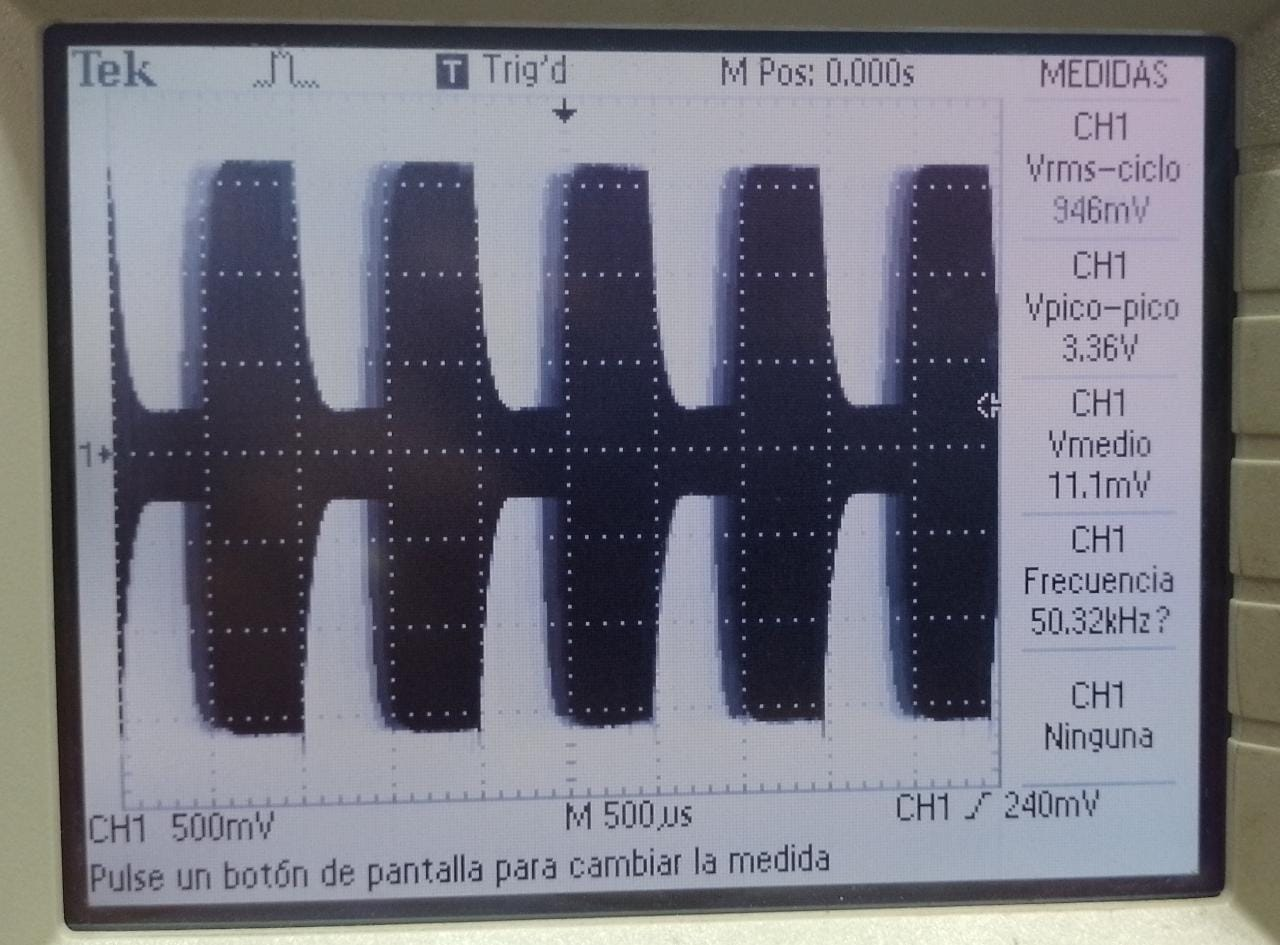
\includegraphics[width=0.44\textwidth]{Imagenes/ActividadPractica/4AnalisisDeUnaSeñalDeAM/Exp4_SeñalAM_CuadradaModulante.jpeg}}
        \caption{Señal AM con onda cuadrada como modulante.}
        \label{fig:SeñalAMConCuadrada}
      \end{figure}

      Finalmente, se hace uso de de las distintas ventanas que posee el menú matemático, para ver la diferencia
      entre cada presentación del espectro de la señal AM en cuestión. En la Figura~\ref{fig:VentanasSeñalAMCuad}
      se puede apreciar lo mencionado.

      \begin{figure}[H]
        \centering
        \begin{subfigure}[H]{0.44\textwidth}
          \frame{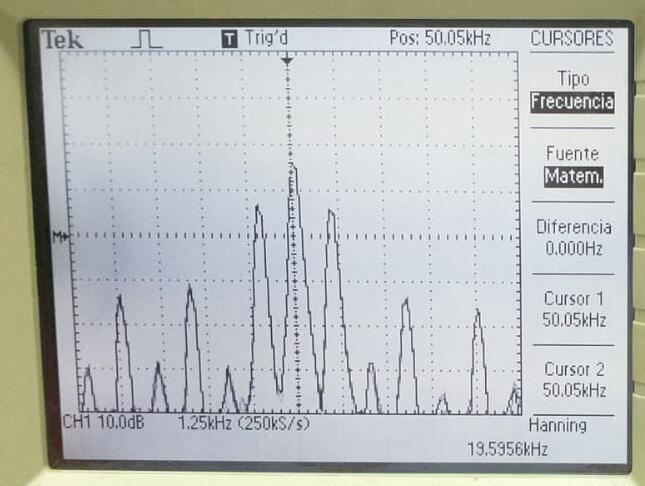
\includegraphics[width=\textwidth]{Imagenes/ActividadPractica/4AnalisisDeUnaSeñalDeAM/Exp4_SeñalRectangularAM_Hanning.jpeg}}
          \caption{Ventana Hanning.}
        \end{subfigure}
        \hfill 
        \begin{subfigure}[H]{0.42\textwidth}
          \frame{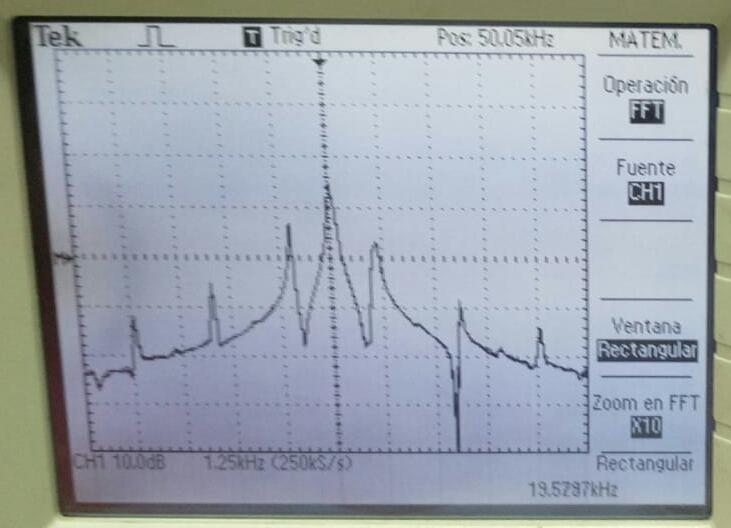
\includegraphics[width=\textwidth]{Imagenes/ActividadPractica/4AnalisisDeUnaSeñalDeAM/Exp4_SeñalRectangularAM_Rectangular.jpeg}}
          \caption{Ventana Rectangular.}
        \end{subfigure}
        \hfill 
        \begin{subfigure}[H]{0.44\textwidth}
          \frame{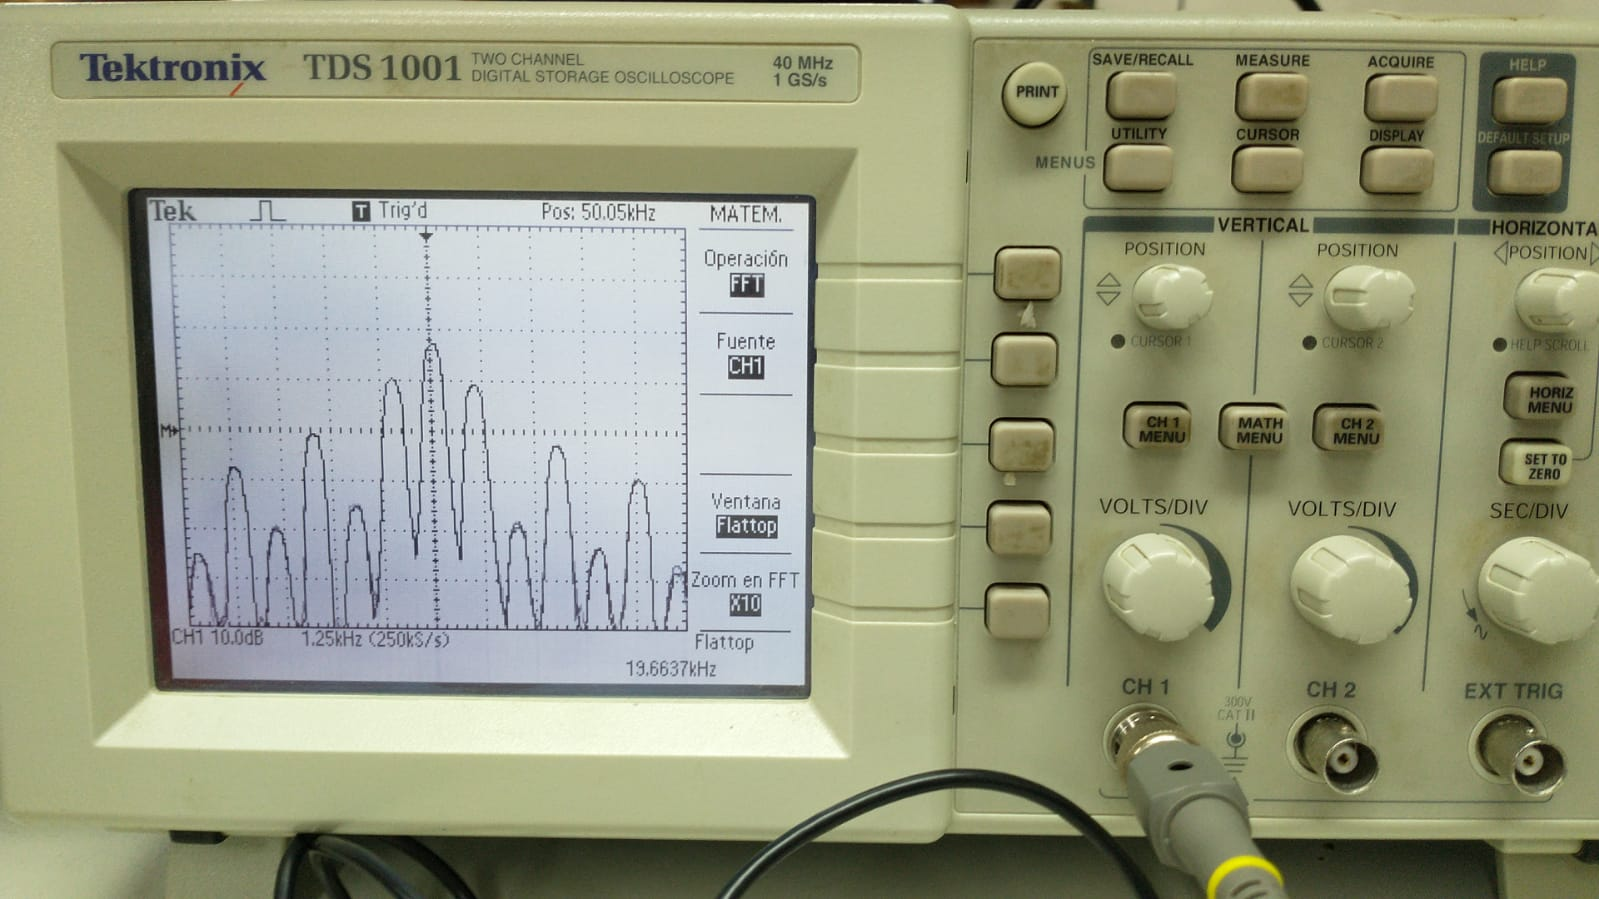
\includegraphics[width=\textwidth]{Imagenes/ActividadPractica/4AnalisisDeUnaSeñalDeAM/Exp4_SeñalRectangularAM_Flattop.jpeg}}
          \caption{Ventana Flattop.}
        \end{subfigure}
      
        \caption{Distintas ventanas de una señal AM con onda cuadrada como modulante.}
        \label{fig:VentanasSeñalAMCuad}
      \end{figure}


    \subsubsection{Señal triangular como modulante}
      De la misma forma que en la sección anterior, se procede a cambiar el generador \textbf{G2} para que 
      inyecte una señal triangular como \textbf{modulante} con la misma frecuencia antes utilizada, 
      respetando la relación de amplitudes previamente configurada. La señal AM obtenida se puede ver en la 
      Figura~\ref{fig:SeñalAMConTriangular}.

      \begin{figure}[H]
        \centering
        \frame{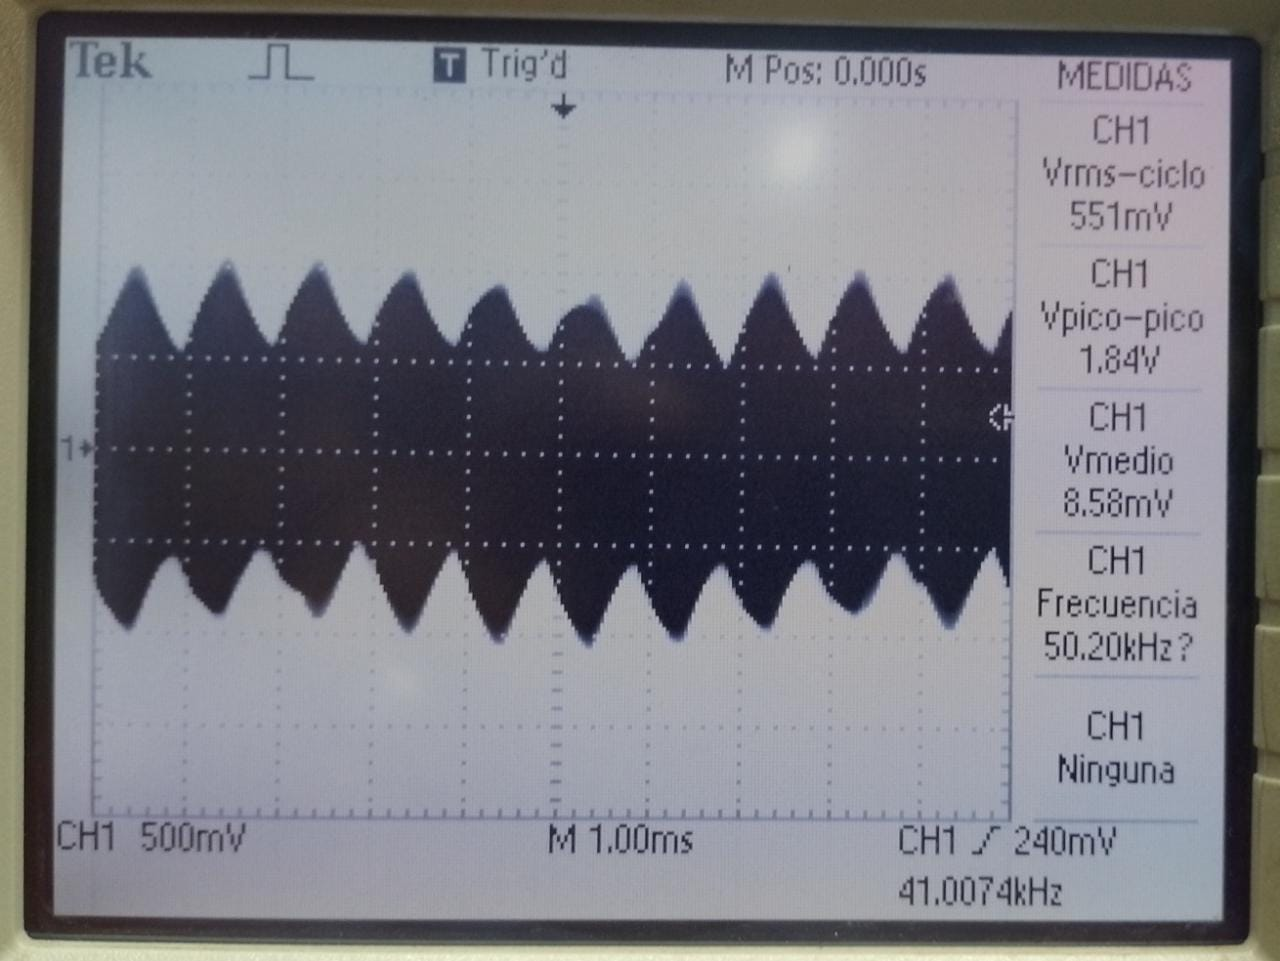
\includegraphics[width=0.44\textwidth]{Imagenes/ActividadPractica/4AnalisisDeUnaSeñalDeAM/Exp4_SeñalAM_TriangularModulante.jpeg}}
        \caption{Señal AM con onda triangular como modulante.}
        \label{fig:SeñalAMConTriangular}
      \end{figure}

      Finalmente, se hace uso de de las distintas ventanas que posee el menú matemático, para ver la diferencia
      entre cada presentación del espectro de la señal AM en cuestión. En la Figura~\ref{fig:VentanasSeñalAMTriang}
      se puede apreciar lo mencionado.

      \begin{figure}[H]
        \centering
        \begin{subfigure}[H]{0.44\textwidth}
          \frame{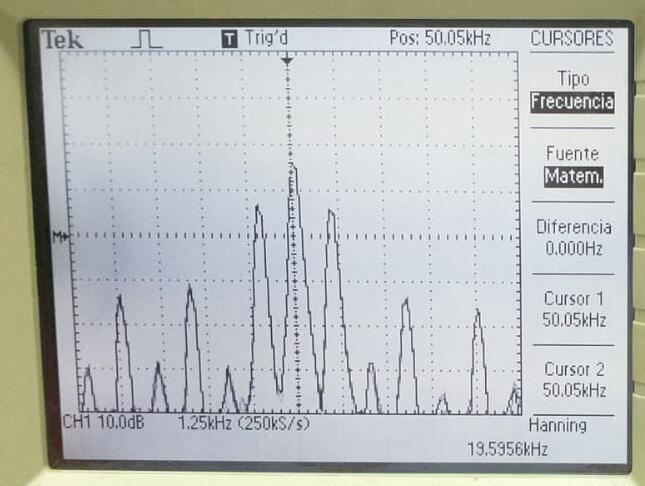
\includegraphics[width=\textwidth]{Imagenes/ActividadPractica/4AnalisisDeUnaSeñalDeAM/Exp4_SeñalRectangularAM_Hanning.jpeg}}
          \caption{Ventana Hanning.}
        \end{subfigure}
        \hfill 
        \begin{subfigure}[H]{0.42\textwidth}
          \frame{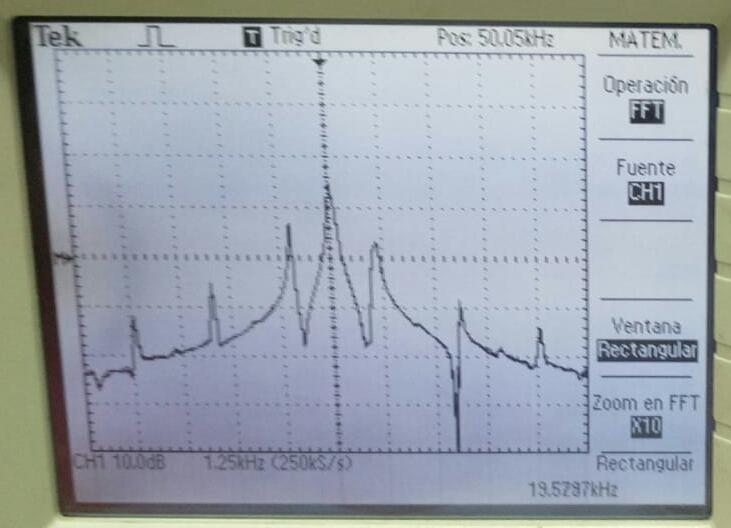
\includegraphics[width=\textwidth]{Imagenes/ActividadPractica/4AnalisisDeUnaSeñalDeAM/Exp4_SeñalRectangularAM_Rectangular.jpeg}}
          \caption{Ventana Rectangular.}
        \end{subfigure}
        \hfill 
        \begin{subfigure}[H]{0.44\textwidth}
          \frame{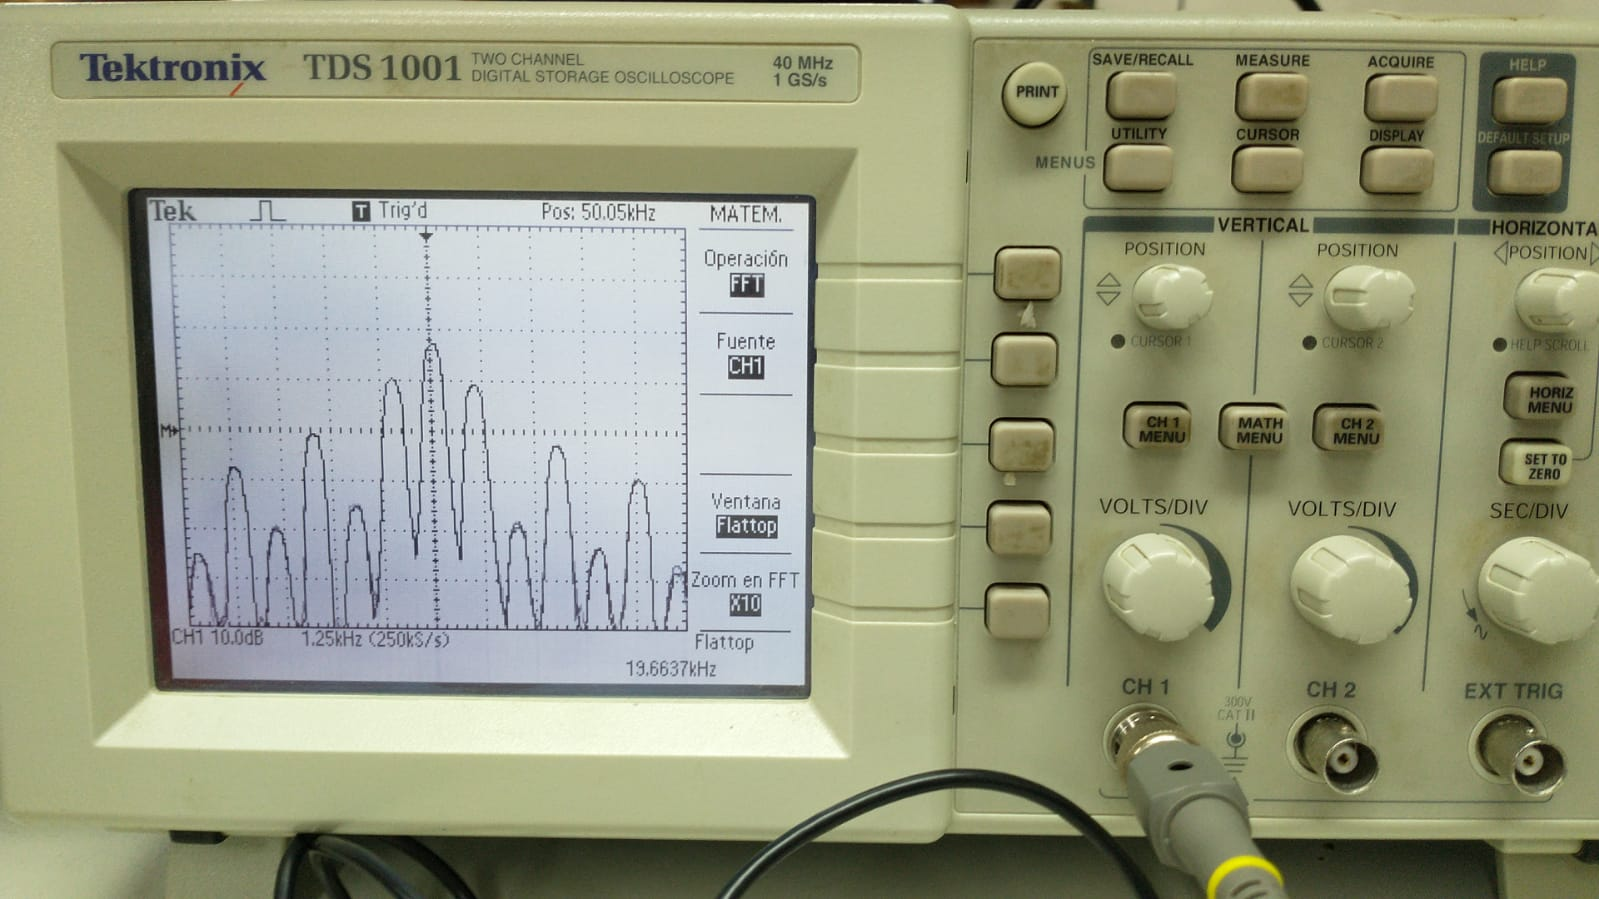
\includegraphics[width=\textwidth]{Imagenes/ActividadPractica/4AnalisisDeUnaSeñalDeAM/Exp4_SeñalRectangularAM_Flattop.jpeg}}
          \caption{Ventana Flattop.}
        \end{subfigure}
      
        \caption{Distintas ventanas de una señal AM con onda triangular como modulante.}
        \label{fig:VentanasSeñalAMTriang}
      \end{figure}

